\chapter{Analýza lesního mikroklimatu}\label{chap:ch1}
V následující části \ref{chap:fyz} popíšeme fyzikální děje odehrávající se poblíž zemského povrchu z pohledu mikrometeorologie a mikroklimatologie. Od jednoduchých ilustračních příkladů se přesuneme k tomu, jaký vliv má na mikroklima topografie \ref{chap:topo} a přítomnost vegetace \ref{chap:veg}. V závěrečné části této kapitoly \ref{chap:measure} popíšeme jak meteorologické podmínky ovlivňují teplotu a jak jsou měřeny, a v \ref{chap:sumavabavorskyles} se podíváme na klima typické pro Národní park Šumava a Bavorský les. V kapitole \ref{chap:statistika} jsme popsali statistické metody využité v kapitole \ref{chap:analysis}.

\section{Fyzikální pohled na děje při povrchu země} \label{chap:fyz}
Nyní popíšeme energetickou bilanci poblíž povrchu země. Pro rovný a téměř homogenní povrch, který můžeme omezit zeshora a zespoda rovinou, platí zjednodušenná rovnice. Tato rovnice vyjadřuje energetickou bilanci \parencite{arya2001}
\begin{gather}\label{eq:bilance}
R_N = H + H_L + H_G + \Delta H_S,
\end{gather}
kde $R_N$ je celková bilance záření, $H$ je tok zjevného tepla z/do atmosféry, $H_L$ je latentní teplo, $H_G$ je tok tepla ze země a $\Delta H_S$ je změna uchovaného tepla za jednotku času na jednotku plochy přes celou hloubku vrstvy. $\Delta H_S$ můžeme také interpretovat jako rozdíl mezi energií dodanou a odevzdanou z vrstvy která nás zajímá. Pak platí pro $\Delta H_S>0$ se vrstva ohřívá a pro $\Delta H_S<0$ se ochlazuje, protože platí, že $H_{in}<H_{out}$. Na jednoduchém případě na obrázku \ref{fig:energy_drylakebed} vidíme vývoj toku energie na povrchu vyschlého jezera. Přes den se povrch ohřívá díky dopadu slunečního záření $R_N>0$, část tepla uniká pod povrch, $H_G<0$ a část ohřívá atmosféru, která sama pouze velmi málo absorbuje záření $H<0$. Naopak v noci vyzařuje povrch dlouhovlnné záření a tím se ochlazuje, tedy $R_N<0$, $H$ je téměř nulové, a zahřáté hlubší vrstvy půdy zpětně ohřívají povrch, $H_G>0$. Po celou dobu jde o suchý povrch, $H_L=0$ \parencite{arya2001}. Většinou ovšem nemůžeme měřit přímo jednotlivé toky tepla.

\begin{figure}
	\centering
	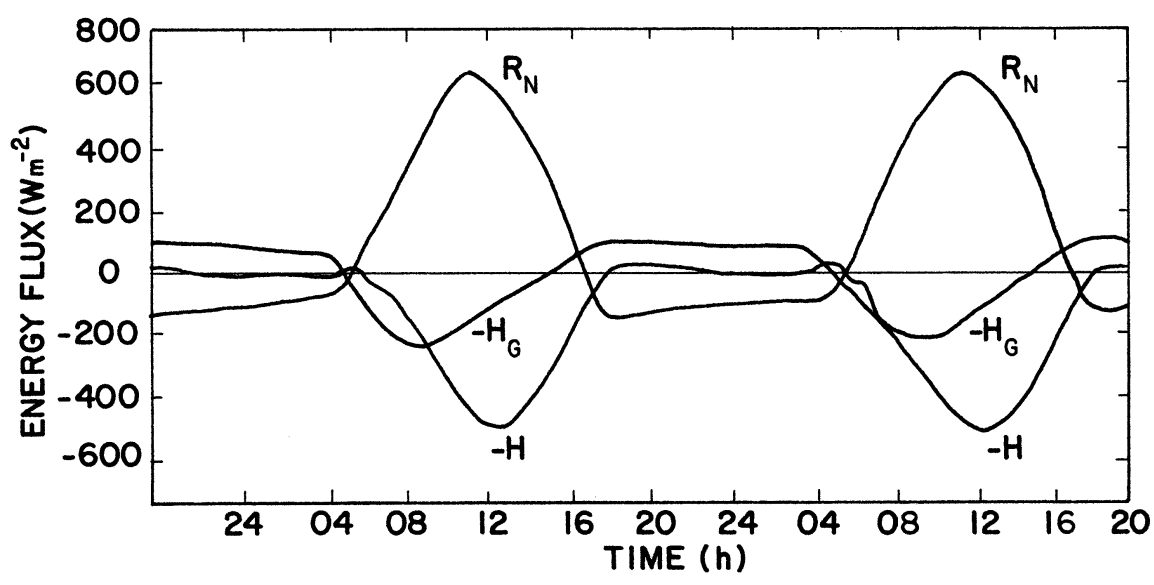
\includegraphics[width=0.95\textwidth]{img/ch1/energy_drylakebed.png}
	\caption{Pozorovaný tok tepla nad vyschlým jezerem El Mirage v Kalifornii 10.-11.6.1950 převzato z \parencite{arya2001}}
	\label{fig:energy_drylakebed}
\end{figure}

\subsection{Vliv latentního tepla}\label{chap:latentheat}
Latentní teplo, které značíme $H_L$, je veličina týkající se změny skupenství látek, v našem případě týkající se vody. Formálně můžeme latentní teplo zavést jako $H_L = T\Delta s$, kde $T$ je teplota, při které dochází ke změně skupenství, a $\Delta s$ je rozdíl mezi molárními entropiemi obou fází \parencite{callen1985}. Za standardního atmosférického tlaku $\SI{1013}{hPa}$ je měrné latentní teplo tání $H_{lT} = \SI{334}{kJ/kg}$ a latentní teplo vypařování $H_{lv} = \SI{2265}{kJ/kg}$. 

Výše jsme analyzovali situaci, kdy šlo o suchý povrch. Pro vlhký povrch se nám situace změní. Část tepla bude absorbována vodou a spotřebována na výpar. Můžeme ovšem mít i opačnou situaci, kdy dochází ke kondenzaci vodní páry a uvolňování latentního tepla. Analogicky můžeme uvažovat situaci v zimě, kdy je přítomná voda v pevném skupenství. V našem zjednodušeném příkladě je tedy přes den $H_L > 0$ a v noci $H_L < 0$. Schématické znázornění můžeme vidět na obrázku \ref{fig:schema}. Velikost jednotlivých toků tepla je ovlivněna mnoha faktory \parencite{arya2001}.

\begin{figure}
\centering
	\begin{tikzpicture}
  % Part a: Day
  \draw (-1,0) -- (4,0);
  \draw[pattern=north east lines] (-1,0) rectangle (4,-0.2);
	\draw[-{Stealth},thick] (1,3) -- (1,0) node[midway,left] {$R_N$};
  \draw[-{Stealth},thick] (2,0) -- (2,2) node[midway,right] {$H$};
  \draw[-{Stealth},thick] (3,0) -- (3,1) node[midway,right] {$H_L$};
  \draw[-{Stealth},thick] (0,-0.2) -- (0,-1) node[midway,left] {$H_G$};
  \node at (2,-2) {(a) Situace ve dne};
	\node at (-0.7,0.25) {\textit{Povrch země}};

  % Part b: Night
  \begin{scope}[xshift=6cm]
    \draw (-1,0) -- (4,0);
    \draw[pattern=north east lines] (-1,0) rectangle (4,-0.2);
    \draw[-{Stealth},thick] (1,0) -- (1,1.5) node[midway,left] {$R_N$};
    \draw[-{Stealth},thick] (2,0.75) -- (2,0) node[midway,right] {$H$};
    \draw[-{Stealth},thick] (3,0.5) -- (3,0) node[midway,right] {$H_L$};
    \draw[-{Stealth},thick] (0,-1) -- (0,-0.2) node[midway,left] {$H_G$};
    \node at (2,-2) {(b) Situace v noci};
  \end{scope}
	\end{tikzpicture}
\caption{Schéma toku tepla ve dne a v noci}
\label{fig:schema}
\end{figure}

Vliv vlhkosti a deště můžeme ilustrovat na takzvaném "oázovém efektu". Oázovým efektem nazýváme situaci, kdy vítr přináší suchý teplý vzduch nad chladnou a vlhkou oblast. Dochází k silnému výparu, který ochlazuje vlivem latentního tepla povrch země. Ve správných podmínkách se může hodnota $H_L$ stát v rovnici \eqref{eq:bilance} i dominantní složkou. Následně máme tok tepla $H$ negativní zatímco $H_L$ je větší a pozitivní. Může se stát, že i tok tepla v půdě $H_G$ změní znaménko, pokud povrch bude chladnější než půda \parencite{arya2001}.

\subsubsection{Albedo}
Energetickou bilanci ovlivňuje i albedo. Albedo je koeficient udávající poměr mezi odraženým a dopadajícím zářením. Nabývá hodnot v intervalu $\langle 0,1\rangle$, kde $0$ znamená, že povrch všechno záření pohlcuje, jde o ideálně černé těleso. Naopak pokud albedo nabývá hodnoty $1$, tak povrch všechno záření odráží. Pro situace, kterými se zabývamé v mikrometeorologii, myslíme albedem většinou odrazivost v konkrétním části spektra a to $\SI{0.15}{\micro m}$ až $\SI{4}{\micro m}$. Vyzařování povrchu země se pak týká delších vlnových délek od $\SI{3}{\micro m}$ až $\SI{100}{\micro m}$. 

Už samotný typ povrchu má na albedo významný vliv. Může dosahovat velmi různých hodnot ať už jde o písek, vodní plochu, půdu bez vegetace nebo například vlhkou půdu. Albedo se také liší s ohledem na typ vegtace. Ilustrační příklady jsou v tabulce \ref{tab:albedo}. Hodnoty jsou závislé i na úhlu dopadu záření, vliv má i výška porostu nebo roční období \parencite{arya2001,alma}.

\begin{table}
\centering\footnotesize\sf
\begin{tabular}{lr}
\toprule
Typ povrchu & Albedo \\
\midrule
Vodní plocha & 0.10-1.00 \\
Čerstvý snih & 0.45-0.95 \\
Suchý písek & 0.35-0.45\\
Vlhký písek & 0.2-0.3\\
Krátký trávník ($\SI{20}{cm}$) & 0.26\\
Delší trávník ($\SI{1}{m}$) & 0.16\\
Opadavý les & 0.1-0.2\\
Neopadavý les & 0.05-0.15\\
\bottomrule
\end{tabular}
	\caption{Výběr různých typů povrchů a odpovídajících hodnot albeda. Převzato z \parencite{arya2001}.}
\label{tab:albedo}
\end{table}

\subsection{Vliv topografie} \label{chap:topo}
V následující části se budeme soustředit na vliv topografie na meteorologické proměnné. Pro standardizované meteorologické stanice je typické, že jsou postavené na posekané travnaté ploše, která není zastíněná a terén není nakloněn. V reálné krajině tohle ovšem neplatí.

\subsubsection{Vliv okraje lesa}
V oblasti okraje lesního porostu je rozhranní v kterém se rychle můžou měnit podmínky. Změny podmínek byly popsány v předchozích odstavcích. Geografická orientace má vliv na to, jak dlouho dopadá denní světlo na toto rozhraní. Množství dopadající energie může být pro okraj lesa orientovaný na jih i několikrát větší, než pro okraj orientovaný na sever. To platí například pro lesy v Evropě. Na rozhraní lesa a otevřené oblasti můžeme dokonce pozorovat vyšší teploty než uvnitř lesa a mimo něj, částečně to může být kvůli sníženému promíchávání vzduchu, větší absorpci slunečního záření, stínění dlouhovlnného záření a nižšímu výparu. Vliv na teplotu má i vítr. Jestliže fouká směrem do lesa, má teplota na okraji lesa tendenci být podobná teplotě mimo les a naopak pro vítr směrem z lesa \parencite{alma}.

\subsubsection{Vliv sklonu a orientace svahu}
Množství slunečního záření, které dopadne na povrch země závisí na mnoha faktorech. Musíme vzít v potaz zeměpisnou šířku, období v roce, denní čas, sklon svahu a orientaci svahu. Například svah mířící na sever s velkým sklonem na severní polokouli, nemusí dostat během zimy po většinu dne žádné sluneční záření. Abychom dostali úplný obrázek musíme započítat i difúzní záření, které je primární složkou záření, pokud je zataženo. Difúzní sluneční záření je složka slunečního záření rozptýlená například atmosférou nebo oblaky a nemá daný směr narozdíl od přímého slunečního záření. Difúzní záření není do takové míry ovlivněné sklonem svahu \parencite{alma}.

\subsubsection{Vliv údolí}
Dalším důležitým faktorem je topografie lokality (kopec, údolí), kterou se zabýváme. Studený vzduch je hustší a tudíž klesá do údolí, kde pak může vznikat kapsa studeného vzduchu. Údolí je typické prostředí, kde můžeme pozorovat inverzi vzduchu. Na dno pak může dopadat menší množství slunečního záření a dlouhovlnné záření může být částečně stíněno okraji údolí. Do údolí hůře proniká vítr, a tudíž je zde snížená turbulence a tím i turbulencí předávané teplo, viz \ref{chap:vlivnaturbulenci}. Všechny tyto faktory mají opačný vliv v případě kopců a obecně vyvýšených míst \parencite{alma}. 

%%%%%%
%Následující odstavce zřejmě nejsou tak důležité pro měřítko mojí práce.
%%%%%%

%\subsubsection{Vliv topografie na vítr}
%Vítr ovlivněný topografií terénu můžeme rozdělit na tři typy podle původu: kompenzační vítr, horský a údolní vítr a vítr spojený se sklonem svahu. V prvním případě jde o vítr způsobený nevyváženým ohřevem zemského povrchu. Na teplejším místě se izobary začnou zvedat, a tím vzniká horizontální gradient tlaku mezi chladnou a teplejší oblastí. Vítr spojený se sklonem svahu má v noci tendenci jít z vyšších nadmořských poloh dolů a naopak během dne. Můžeme mít také situaci, kdy pozorujeme údolí, které se zároveň svažuje. Zde už je situace složitější.

%Při svítání se začíná povrch údolí ohřívat. Vzduch u strany údolí stoupá nahoru, ale údolní vítr stále ještě fouká směrem dolů. Během dne údolní vítr oslabuje, až dojde k obrácení jeho směru a údolím fouká nahoru. Později odpoledne vítr po svazích začne ustávat, a fouká pouze údolní vítr do vyšších nadmořských výšek. Následně chladnější vzduch ze stran údolí začne klesat, a v noci nakonec údolní vítr začne opět vát dolů stejně jako vítr po svazích údolí. Toto popisuje ukázkovou situaci za letního dne bez oblačnosti. Ilustraci k tomuto popisu můžeme vidět na obrázku \ref{fig:valley_winds}

%\begin{figure}
%	\centering
%	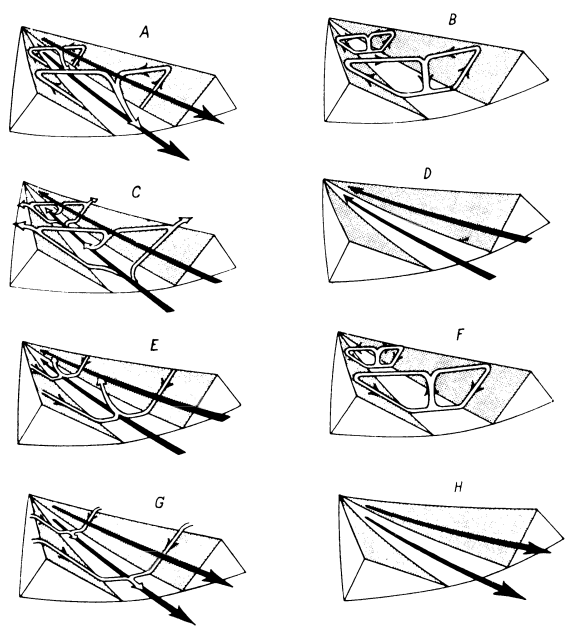
\includegraphics[width=0.95\textwidth]{img/ch1/valley_winds.png}
%	\caption{Typický průběh proudění napříč letním dnem. Převzato z \parencite{alma}.}
%	\label{fig:valley_winds}
%\end{figure}

%Vítr ovlivněný topografií může mít další podoby, které ovšem pro tuto práci nejsou zásadní. Můžeme zmínit mořský vánek mezi střídavě rychle se ohřívajícím pobřežím a relativně studenému moři ve dne, a rychle chladnoucím pobřeží a relativně teplému moři v noci. Významný vítr spojený s horskou topografií pak dostává různé názvy jako fén v Alpách nebo mistrál ve Francii \parencite{alma}.

\subsection{Vliv vegetace} \label{chap:veg}
\subsubsection{Vliv na tok tepla}
Do členů v rovnici \ref{eq:bilance} můžeme zahrnout i růst vegetace. V tu chvíli musíme počítat s významnou prostorovou závislostí všech toků tepla a záření. Následně jsou pro nás nejdůležitější hodnoty $R_N$, $H$ a $H_L$ nad vegetací. $\Delta H_S$ se skládá ze dvou částí a to změny zjevného tepla ve vzduchu nebo vegetaci a změny energie biochemického původu skrze fotosyntézu a přesunu oxidu uhličitého. Latentní teplo se skládá z výparu a kondenzace vody a také z transpirace vody listy rostlin, mluvíme o evapotranspiraci. Při měření je obtížné od sebe transpiraci a evaporaci oddělit. Například během růstu plodin zpočátku je hlavní složka evapotranspirace výpar, ale později plodina zakrývá větší plochu povrchu tak se stává majoritní složkou transpirace a má významný vliv na energetickou bilanci \parencite{arya2001, evapotranspiration}. 

Vliv na celkový tok energie má i výška porostu, například v lese může být nezanedbatelné množství tepla uchovaného v úrovni vegetace, které může způsobit, že prostředí reaguje pomalu na změnu teploty a jiných veličin. Pro suchý porost může uchovaná energie dosahovat až $\SI{7}{\%}$ celkového toku energie skrze dopadající záření. Situace se ovšem pro vlhký porost obrací, a uchovaná energie může být záporná. Míru uchování energie v porostu měříme v $\si{}{\text{cal}\cdot \text{cm}^{-2}\cdot \text{min}^{-1}}$. Typicky je kladná během dne, kdy se vzduch ohřívá a záporná v noci. Například oblačnost změnšuje amplitudu denního chodu uchované energie \parencite{alma}. 

Podle \parencite{alma} ovlivňuje teplotu hustota porostu. Měříme-li teplotu v řidším lese, a sledujeme její průběh od země až po koruny stromů, tak teplo snadněji prochází vegetací. Při zemi budou podobné teploty jako ve výšce několika metrů nebo až v korunách stromů. Naopak, pokud se nacházíme v hustějším lese, tak bude teplota růst dříve v oblasti korun stromů a teplota při zemi může stoupat o několik hodin později a také dosahovat nižších denních maximálních hodnot. V noci také může v řidším lese docházet k inverzi teplot, zatímco v hustějším lese budou teploty podobné napříč porostem. 

Tok tepla v lese je ovlivněn i větrem. Jestliže fouká silný vítr, dochází k přenosu tepelné energie z nebo do lesního porostu. Rychlost přenosu může opět záviset na hustotě lesa \parencite{alma}. 

\subsubsection{Vliv na míru turbulence}\label{chap:vlivnaturbulenci}
Turbulence vzduchu je zodpovědná za přenos hmoty, tepla a hybnosti v blízkosti povrchu země. Bez turbulence by promíchávání probíhalo na molekulární úrovni a řádově menším měřítku. Turbulenci ovlivňuje typ povrchu přes který se vzduchová hmota pohybuje. Například nad sněhovým polem nebo klidnou vodní plochou bude vzduch proudit s menší turbulencí a pro les s vegetací v bylinném patře naopak vyšší \parencite{alma}. 

\subsubsection{Vliv na rychlost větru}\label{chap:vlivnavitr}
Přítomnost vegetace ovlivňuje rychlost větru a přenos vzduchových hmot z/do oblasti porostu. Profil větru může být v lese nehomogenní. Například koruny stromů můžou rychlost větru výrazně snižovat. Zatímco rychlost větru blíž povrchu může být vyšší, pokud blízko země nejsou menší stromy, keře nebo jiné překážky. To má pak vliv na teploty uvnitř porostu, které se mohou více podobat teplotám ve volném vzduchu. Z toho plyne, že vliv na rychlost větru má i přítomnost listů a jejich absence v zimě \parencite{alma}. 

\subsubsection{Vliv na vlhkost vzduchu}
V předchozím odstavci jsme zmínili transpiraci flóry, která slouží jako zdroj vodní páry. Ukázková situace v jehličnatém lese může vypadat tak, že tlak vodní páry dosahuje dvou maxim a to při povrchu půdy z důvodu nižšího promíchávání vzduchu a výparu a v oblasti korun stromů kvůli listům. Druhé maximum bývá menší, kvůli promíchávání se suchým vzduchem nad korunami stromů \parencite{alma}. 

\subsubsection{Vliv na rosu}
Přítomnost stromů také ovlivňuje rozložení a množství rosy v jejich okolí. Tam kde je porost hustší, tak dopadá na zem v noci méně rosy díky stínění povrchu porostem. Dále pak porost brání úniku dlouhovlnného záření, což způsobuje pomalejší pokles teploty během večera. Díky relativně vyšším večerním teplotám se sníží množství rosy. Nad ránem se naopak v lese drží déle nižší teploty, protože porost brání dopadu slunečního záření a tím setrvává rosa na zemi delší dobu. Při měření množství ranní rosy v různé vzdálenosti od kmene stromu s celkovým zápojem o poloměru $\SI{5.2}{m}$ bylo pozorováno, že množství rosy roste strmě do zhruba $\SI{2}{m}$ od kmene a dále pomaleji. Doba, po kterou zůstala rosa na zemi, také se vzdáleností rostla a od vzdálenosti $\SI{4}{m}$ lehce klesala \parencite{alma}.

\subsubsection{Vliv na déšť}
Typ porostu (listnaté/jehličnaté lesy) má vliv na distribuci deště. Největší množství vody se objevuje na vnějším okraji ohraničeném korunou stromu. Stromy bez listů mají na prostorové rozložení srážek pouze minimální vliv. Pod jehličnaté stromy dopadá pouze $\SI{60}{\%}$ až $\SI{90}{\%}$ srážek, a v oblasti okraje korun dopadá o $\SI{10}{\%}$ až $\SI{20}{\%}$ více srážek než v místě bez porostu. Tento rozdíl je způsoben tím, že část vody stéká po větvích a listech, kde listy a jehličí nejdále od stromů slouží jako okap. Konkrétní hodnoty jsou ovlivněné druhem dřeviny a roční dobou. Lesní porost také při slabém dešti může úplně zabránit dopadu srážek na půdu. Množství vody, které takto dokážou stromy zachytit, se může pohybovat od $\SI{1}{mm}$ do $\SI{3}{mm}$. Část vody je také ztracena výparem z povrchu listu, který je podpořen výraznějším promícháváním vzduchu v oblasti horní části korun stromů \parencite{alma}.

\subsubsection{Vliv na sníh}\label{chap:vlivnasnih}
Množství sněhových srážek, které dopadnou na zem v lesním porostu záleží na několika faktorech. Jestliže jde o mokrý sníh, pak snadno zůstává v korunách stromů. Takto může být v korunách zachyceno až $\SI{10}{cm}$ sněhu. Suchý sníh naopak snáze dopadne na zem. Množství zachyceného sněhu závisí také na typu vegetace, jestli jde o listnaté nebo jehličnaté stromy, případně o jaký druh stromu. Na jaře taje sníh v lese pomaleji a jeho přítomnost je pro místní klima velmi důležitá, protože funguje jako zásobník vody \parencite{alma}.

\subsection{Rozdíl mezi teplotou při povrchu země a ve standardní výšce}
Teplota vzduchu se typicky myslí ve výšce $\SI{1.25}{m}$ až $\SI{2}{m}$ \parencite{wmo2021}, přičemž stanice Churáňov a ostatní automatické stanice použité v této práci měří teplotu vzduchu ve $\SI{2}{m}$ \parencite{churanov}. Jestliže máme situaci, kdy na povrch svítí přímé sluneční záření, tak se můžou poblíž povrchu vyskytovat výrazné gradienty teplot a to $\SI{10}{K/mm}-\SI{20}{K/mm}$. Tyto výrazné gradienty jsou ovlivněné mnoha faktory jako například druh povrchu nebo jeho vlhkost a další, které byly diskutovány výše \parencite{arya2001}. 

\section{Analýza faktorů ovlivňující teplotu vzduchu v lesním porostu}
V předchozích odstavcích jsme diskutovali vliv vegetace a topografie na různé meteorologické proměnné. Tuto souvislost v následující části budeme aplikovat na konkrétní studii týkající se výzkumných ploch po střední Evropě.

\subsection{Vliv topografie a struktury krajiny na teplotu}
Při hledání vlivu topografie na rozdíl mezi teplotou v lesním porostu a na nejbližší meteorologické stanici ve střední Evropě byly ve výzkumu \parencite{ZellwegerFlorian2019Sdou} použity následující prediktory:
\begin{itemize}
	\item Plocha pokrytá lesním porostem v okruhu $\SI{250}{m}$ vyjádřená v procentech.
	\item Vzdálenost k okraji lesa.
	\item Vzdálenost k nejbližšímu pobřeží.
	\item Výška nad mořem. 
	\item Sklon svahu k severu/jihu.
	\item Sklon svahu vzhledem k horizontální/vodorovné rovině.
	\item Index udávající zda-li jde spíše o údolí nebo vyvýšené místo.
	\item Slabšími prediktory pak bylo sklon svahu k severu/jihu, sklon svahu a hodnota udávající zda-li jde spíše o údolí nebo vyvýšené místo.
\end{itemize}
U plochy pokryté lesním porostem nebyla nalezena spojitost s rozdílem teplot. Vzdálenost k okraji lesa byla nevýznamným prediktorem. Vzdálenost k nejbližšímu pobřeží a vyška nad mořem byly nejsilnějšími prediktory, zároveň jde ovšem o silně korelované veličiny. Sklon svahu k severu/jihu, sklon svahu k horizontální/vodorovné rovině a index údolí/vyvýšeného místa byly slabšími prediktory.

Tyto výsledky ovšem nejsou konzistentní mezi různými studiemi. Například podle \parencite{GreiserCaroline2018Mmmi} je plocha pokrytá lesním porostem důležitou hodnotou a může vést ke zvýšení minimální denní teploty až o $\SI{3}{\degree C}$, zároveň \parencite{GreiserCaroline2018Mmmi} ukázali, že vzdálenost k okraji lesa je středně silným prediktorem.

\subsection{Vliv porostu na teplotu}
Druhou skupinou prediktorů, kterou se \parencite{ZellwegerFlorian2019Sdou} zabýval, byly proměnné týkající se porostu v blízkém okolí čidla.
\begin{itemize}
	\item Zápoj, neboli míra uzavřenosti korun stromů, kde $\SI{0}{\%}$ znamená, že obloha není stromy vůbec zakrytá a $\SI{100}{\%}$, že je úplně zakrytá.
	\item Otevřenost porostu vyjádřená jako část viditelné oblohy.
	\item Plocha koruny stromů.
	\item Procento plochy pokryté dřevinami s průměrem větším než $\SI{7.5}{cm}$.
	\item Výška stromu, na kterém bylo čidlo upevněno.
	\item Schopnost porostu vytvářet stín podle typu dřeviny.
\end{itemize}
Zápoj má pro hodnoty nižší než $\SI{89}{\%}$ záporný vliv, pro vyšší hodnoty pak neutrální až lehce kladný vliv. Otevřenost porostu a plocha koruny stromů má záporný nelineární vztah k maximální teplotě. Procento plochy pokryté dřevinami je pouze slabým prediktorem. Výška stromu naopak souvisí s rozdílem maximální teplot kladně, ale opět zde vztah není příliš silný. Schopnost porostu vytvářet stín je středním prediktorem rozdílu maximálních teplot.

\subsection{Vliv meteorologických podmínek na teplotu}\label{chap:vlivmeteo}
Jak bylo zmíněno v předchozí části, tak na rozdíl mezi teplotou mimo porost a v lese má vliv mnoho faktorů od topografických po konkrétní typ porostu. Tyto faktory se dají vyjádřit mnoha různými prediktory, jejichž vliv můžeme sledovat. Aktuální stav počasí je další faktorem, který ovlivňuje naměřené teploty. Mezi takové faktory patří oblačnost, vlhkost, sněhová pokrývka, srážky, rychlost větru a insolace, s kterými budeme dále pracovat v kapitole \ref{chap:analysis}.

Při zvýšené \textit{oblačnosti} dopadá na zem více rozptýleného záření a povrch země se neohřívá přes den tak rychle, stejně tak oblačnost přes noc snižuje únik dlouhovlnného záření, a tedy obecně snižuje amplitudu denních teplot. Tento pokles můžeme vidět na obrázku \ref{fig:diurnaltemp} \parencite{arya2001}.

\begin{figure}
	\centering
	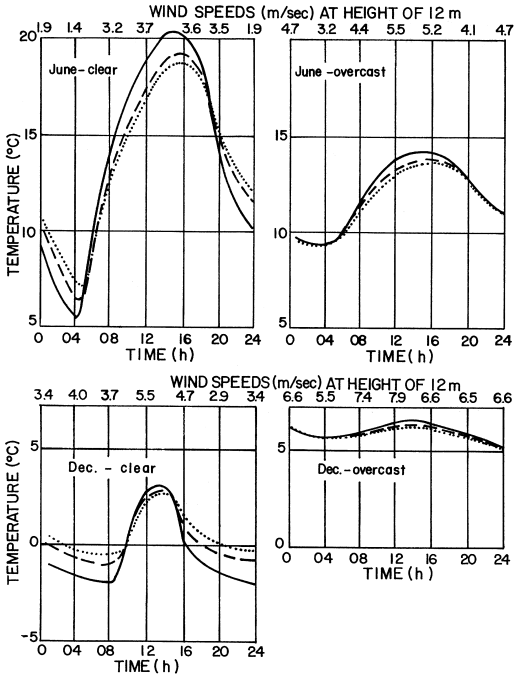
\includegraphics[width=0.95\textwidth]{img/ch1/diurnaltemp.png}
	\caption{Denní vývoj teploty ve třech výškách (plná čára $\SI{1.2}{m}$, čárkovaná $\SI{7}{m}$ a tečkovaná $\SI{17}{m}$) v jižní Anglii pro jasnou a zataženou oblohu a pro červnové a prosincové teploty. Převzato z \parencite{arya2001}}
	\label{fig:diurnaltemp}
\end{figure}

\textit{Vítr} napomáhá promíchávání ohřívaného vzduchu u zemského povrchu s vyššími vrstvami, a tedy typicky dochází při silnějším větru k poklesu teplotního gradientu nad zemí \parencite{arya2001}.

\textit{Sníh} má nízkou tepelnou vodivost. Pod sněhovou pokrývkou tedy v zimě typicky dochází k nárůstu teplot. Zatímco na povrchu sněhu můžou teploty klesat hluboko pod bod mrazu, sníh izoluje zemský povrch a teploty pod ním se můžou blížit nebo i lehce přesahovat $\SI{0}{\celsius}$. Studie z oblasti Altajského pohoří popsala rozdíl teplot mezi zemským povrchem a horní hranicí sněhové pokrývky (o výšce $\SI{0.5}{m}$) až $\SI{12.8}{\degree C}$. Vyšší teploty pod sněhovou pokrývkou využívají různé organismy pro přežití v zimě, viz. obrázek \ref{fig:snowtempaltai} \parencite{hirakawahirofumi2018}. Zatímco na rozhraní vzduch-sníh kolísají teploty od $\SI{0}{\degree C}$ téměř k $\SI{-30}{\degree C}$, tak s hloubkou nejenže amplituda dramaticky klesá, ale také jsou teploty bez výjimky vyšší. Dále můžeme vidět, že výkyvy teplot, ať už dané denním chodem nebo změnou počasí, mají ve sněhové pokrývce zpoždění, které se prodlužuje s výškou sněhu \parencite{zhangwei2021}. S rostoucí mocností sněhu klesá teplotní gradient uvnitř sněhové pokrývky, viz. obrázek \ref{fig:snowlapserate}. Přítomnost sněhu snižuje teplotu na rozhraní sníh-atmosféra \parencite{zhangwei2021}.

\begin{figure}
	\centering
	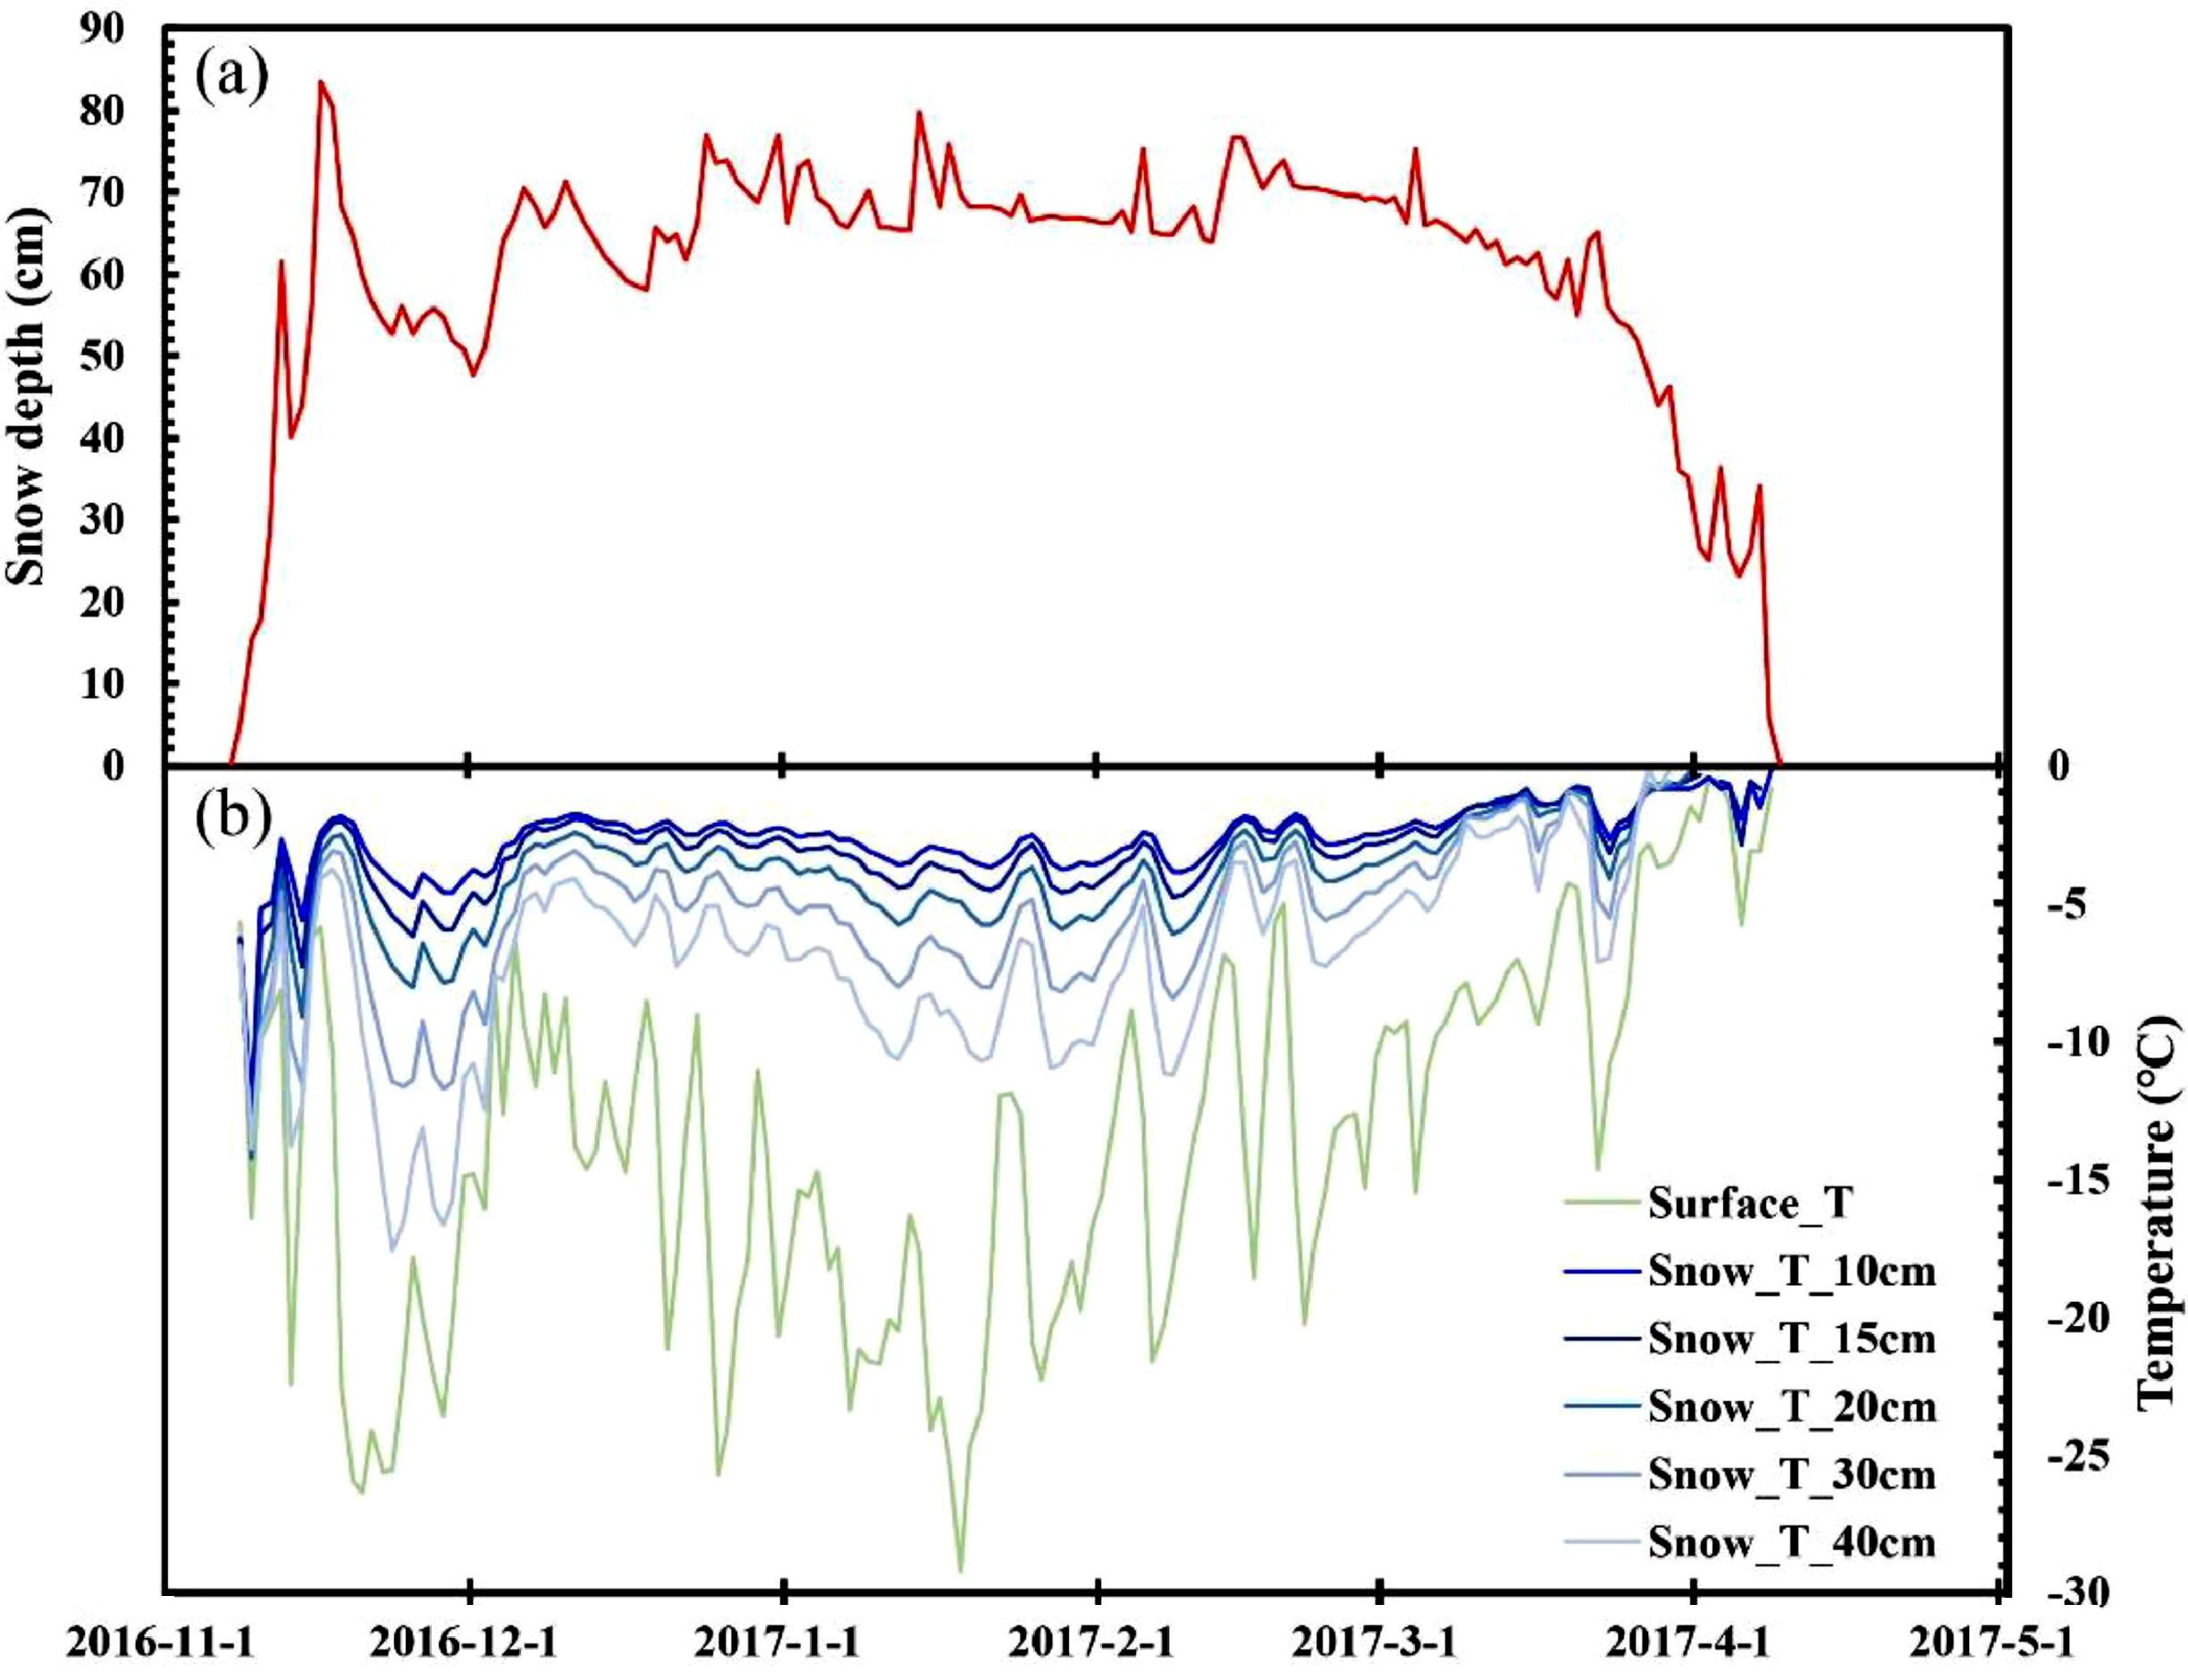
\includegraphics[width=0.95\textwidth]{img/ch1/snowtempaltai.png}
	\caption{Sezónní vývoj teplot pod sněhovou pokrývkou pro $\SI{10}{cm}$, $\SI{15}{cm}$, $\SI{20}{cm}$, $\SI{30}{cm}$, $\SI{40}{cm}$ nad rozhraním půda-sníh a na povrchu sněhu. Data se týkají období od listopadu 2016 do dubna 2017 pozorovaných na Altaji. Převzato z \parencite{zhangwei2021}.}
	\label{fig:snowtempaltai}
\end{figure}

\begin{figure}
	\centering
	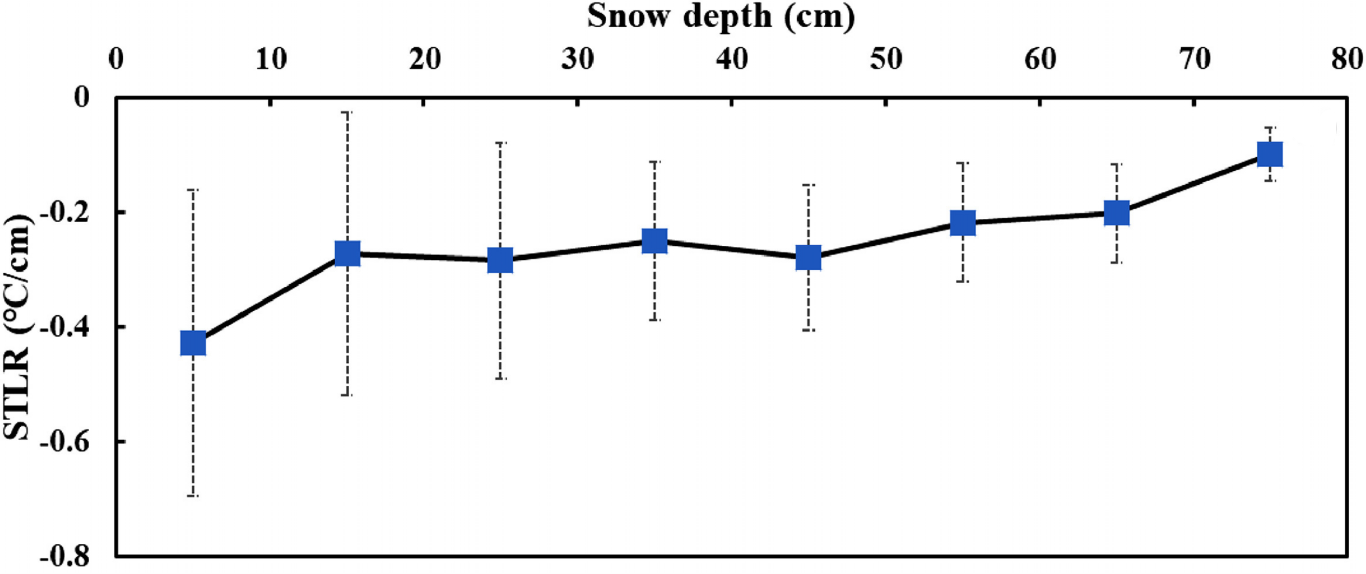
\includegraphics[width=0.95\textwidth]{img/ch1/snowlapserate.png}
	\caption{Teplotní gradient uvnitř sněhové pokrývky v závislosti na její mocnosti. Měřeno na Altaji od listopadu 2011 do dubna 2018. Převzato z \parencite{zhangwei2021}.}
	\label{fig:snowlapserate}
\end{figure}


%%%%%
%Prý následující odstavec není moc relevantní
%%%%%
%Vlhkost vzduchu je pro teplotní gradient v atmosféře důležitou hodnotou. Z hydrostatické rovnice a Poissonových rovnic můžeme odvodit následující vztah\parencite{jakvznikapocasi}
%\begin{gather*}
%-\frac{\text{d}t}{\text{d}z} = \frac{g}{c_p}\frac{T}{T_v},
%\end{gather*}
%kde $T$ je teplota v kelvinech, $T_v$ je virtuální teplota, $g$ je gravitační zrychlení a $c_p$ je měrné teplo při stálém tlaku. Pak pro suchý vzduch, kde $T=T_v$, dostáváme teplotní gradient $-\frac{\text{d}t}{\text{d}z} = \frac{g}{c_p} = \SI{0.98}{\degree C/100 m}$. Pro stoupající vlhký vzduch je ovšem situace jiná, při výstupu dochází k expanzi, která se děje na úkor vnitřní energie vzduchu. Při chladnutí ve vlhkém vzduchu kondenzuje voda a uvolňuje se skupenské teplo, a tudíž je teplotní gradient menší než v suché atmosféře. Tento gradient závisí na tlaku a teplotě vzduchu. Při tlaku $\SI{1000}{hPa}$ nabývá hodnot $\SI{0.76}{\degree C/100 m}$, $\SI{0.65}{\degree C/100 m}$ a $\SI{0.53}{\degree C/100 m}$ pro $\SI{-10}{\degree C}$ resp. $\SI{0}{\degree C}$, resp. $\SI{10}{\degree C}$\parencite{jakvznikapocasi}.

Kapalné \textit{srážky} vedou k nárůstu vlhkosti, jejíž vliv je diskutován výše. Prudký nárůst latentního tepla při výparu může výrazně ovlivnit energetickou bilanci poblíž povrchu, jak bylo nastíněno v části \ref{chap:latentheat}. Dále se srážkami typicky roste oblačnost, a tedy klesá množství slunečního záření dopadajícího na zem. Studie zabývající se korelací srážek a teploty v Evropě na téměř 100 stanicích zjistila, že v zimě na většině území je významná pozitivní korelace mezi množstvím srážek a teplotou. Pro oblast České republiky a Šumavy je korelace o něco menší a to $0.2$. Pro letní období je pak naopak záporná, tedy s větším množstvím srážek klesají teploty, konkrétně jde o hodnotu korelace okolo $-0.4$ \parencite{maddenroland1978}.

\section{Popis měření meteorologický veličin} \label{chap:measure}
\subsection{Měření na meteorologických stanicích}\label{chap:meteostations}
Teplota vzduchu by podle Světové meteorologické organizace (WMO) měla být měřena ve výšce $\SI{1.25}{m}$ až $\SI{2}{m}$ \parencite{wmo2021}. V České republice Český hydrometeorologický ústav provozuje celou řadu meteorologických stanic různého charakteru s různými měřenými meteorologickými proměnnými. Stanice by měla být na trávníku nikoliv například na asfaltu a měření probíhají v pravidelných intervalech. Na stanicích jsou měřeny veličiny jako například, vlhkost, výška sněhu, část zatažené oblohy, tlak a další \parencite{chmustanice}. Meteorologická stanice Churáňov, která je pro naše zpracování dat nejdůležitější, je označována za takzvanou automatizovanou stanici. Měření probíhá v souladu s metodickými doporučeními WMO \parencite{chmustanice2}.

Automatické stanice dovolují pravidelné měření většího množství dat než by bylo možné manuálně. Pomocí automatických stanic je možné měřit v místech, která jsou hůře přístupná. Navíc nám automatické stanice dovolují hustější staniční síť. Automatizace má ovšem i svá omezení pokud jde o klasifikaci jevů nebo určování typu oblačnosti, zde je expertíza meteorologa nebo meteoroložky nezbytná \parencite{automatisation}.

\subsection{Měření v terénu pomocí čidel}
Pomocí meteorologických stanic není možné získat detailní informace o teplotě a dalších veličinách na malých prostorových škálách. Standardní meteorologické stanice nejsou určeny k měření teploty v lesním porostu. Data použitá v této práci jsou měřená pomocí TMS (Temperature-Moisture-Sensor) logger. Kromě čidel jako například Thermochron iButtons, je možné využít radiometrie a z vyzářeného záření z povrchu pomocí Stefan-Boltzmannova zákona spočítat teplotu povrchu. Radiometrie má ovšem své omezení pokud chceme znát teplotu v lesním porostu, kvůli stínění. 

\subsubsection{TMS4 a T1 logger} \label{chap:loggers}
Čidlo TMS4 logger používané pro sběr dat vědci a vědkyněmi z Botanického ústavu Akademie věd České republiky. Toto čídlo je konstruováno tak, aby měřilo podmínky, které ovlivňují malou bylinu. Je tedy vysoké $\SI{15}{cm}$ a sahá do hloubky $\SI{14}{cm}$. Je opatřeno třemi teplotními senzory ve výškách $\SI{15}{cm},\ \SI{0}{cm},\ \SI{-8}{cm}$. Až do hloubky $\SI{14}{cm}$ je měřena volumetrická půdní vlhkost. Všechny hodnoty jsou měřeny v 15 minutových intervalech. Horní část data loggeru je opatřen optickým stíněním z bílého plastu chránící horní senzor před přímým slunečním zářením. Podobně je odstíněn i senzor při povrchu země. 

Teplotní senzor měří s přesností $\SI{\pm 0.5}{\degree C}$ a funguje v intervalu $\SI{-55}{\degree C}$ až $\SI{125}{\degree C}$. Měření volumetrické půdní vlhkostí je založené na time-domain-transmission (TDT), kdy jsou skrze obvod vysílány elektromagnetické pulzy a množství detekovaných pulzů je přímo úměrné vlhkosti. 

Při srovnání TMS4 loggeru se standardní meteorologickou stanicí typu METEOS 5 byla pozorována větší variabilita u teplot v $\SI{15}{cm}$ než ve $\SI{2}{m}$. TMS4 logger byl instalován na krátkém posekaném trávníku, tři metry od stanice, a rozdíl teplot při hodinovém měření se pohyboval od $\SI{+8.5}{\degree C}$ do $\SI{-6.1}{\degree C}$. Průměrné denní teploty naměřené z TMS4 loggeru byly systematicky nižší, průměrný rozdíl ovšem pouze $\SI{-0.58}{\degree C}$, v zimě jsou tyto rozdíly větší a to $\SI{-2.02}{\degree C}$ až $\SI{0.6}{\degree C}$. Opačný trend pak můžeme pozorovat, pokud není teplotní senzor v $\SI{15}{cm}$ odstíněn plastovým krytem. V létě byly teploty nižší až o $\SI{5.08}{\degree C}$, ale v zimě byly podobné. Teploty z půdních senzorů jak TMS4 loggeru tak stanice METEOS 5 se lišily velmi málo, rozdíl mezi naměřenými teplotami byl zřejmě způsoben primárně polohou senzorů a použitým stíněním než jejich typem. Rozdíly mezi naměřenými teplotami nad zemí byly ještě výraznější pro proměnné, které jsou často používány v ekologických studiích, jako například kvantily extrémních teplot \parencite{WildJan2019Caer}. 

Data měřená při povrchu země jsou na některých místech doplněna stejnými teplotními senzory ve výšce $\SI{2}{m}$ upevněnými na kmenu stromu a také opatřena plastovým stínítkem.

\subsection{ERA5}\label{chap:era5}
Copernicus Climate Change and Atmosphere Monitoring Services provádí atmosférickou reanalýzu. ERA5 je pátou verzí této reanalýzy s daty od roku 1940 \parencite{era5}. Data s desítkami veličin jsou dostupná pro každou hodinu s rozlišením $\SI{0.5}{\degree}$, konkrétně budeme používat produkt "ERA5 hourly data on single levels from 1940 to present". Tyto data využijeme v kapitole \ref{chap:analysis} pro doplnění chybějících hodnot oblačnosti ze staničních měření.

\subsection{Výpočet insolace}\label{chap:insolation}
Insolace je množství záření dopadajícího na horní část zemské atmosféry. Insolace záleží na denní době, roční době a zeměpisné šířce. Okamžitá insolace je dána následujícím vztahem \parencite{insolace}
\begin{gather}\label{eq:insolace}
Q = S_0\left(\frac{d_0}{d}\right)^2\left(\sin\phi\sin\delta + \cos\phi\cos\delta\cos h\right),
\end{gather}
kde $S_0$ solární konstanta, $d_0$ je průměrná vzdálenost Země od Slunce, $d$ je aktuální vzdálenost Země od Slunce, $\phi$ je zeměpisná šířka, $\delta$ je deklinační úhel Slunce, $h$ je hodinový úhel Slunce. Tento vzoreček platí pouze pro den, nikoliv v noci, kdy je $Q=0$. Hodinový úhel Slunce spočteme následovně: \parencite{hourangle}
\begin{equation}
	\begin{split}
		h &= 15^{\circ}\left(\text{LST}+\text{offset}/60-12\right)\\
		\text{offset} &= \text{eot} + \text{longV}\\
		\text{eot} &= 229.18\cdot(0.000075+0.001868\cos(\gamma)-0.032077\sin(\gamma)\\
		& -0.014615\cos(2\gamma)-0.040849\sin(2\gamma))\\
		\text{longV} &= 4\cdot\text{longitude}\qquad \gamma = \frac{2\pi}{365}\left(t - 1 + \frac{\text{hour}-12}{24}\right),
	\end{split}
\end{equation}
$\text{LST}$ je místní sluneční čas, ke kterému přičteme korekci způsobenou eliptickou dráhou okolo země a skloněním zemského osy a korekci zahrnující to na jaké zeměpisné šířce se nacházíme. Faktor $\gamma$ je část roku vyjádřena ve zlomku.
Deklinační úhel s předpokladem, že Země obíhá po kružnici: \parencite{declinationangle}
\begin{gather*}
\delta = \SI{-23.45}{\degree} \cdot \cos\left(\frac{360}{365}\cdot(t+10)\right),
\end{gather*}
$t$ je den v roce, tedy pro 1. leden $t=1$. Vzdálenost Země od Slunce pro \eqref{eq:insolace} je daná vztahem \parencite{sunearthdist}
\begin{gather*}
d = 1-0.01672\cdot \cos\left(0.9856\cdot(t-4)\right)
\end{gather*}



\section{Národní park Šumava a Bavorský les} \label{chap:sumavabavorskyles}
Čidla TMS logger z kterých pocházejí data použitá v této práci se nacházejí v oblasti Národního parku Šumava o rozloze $\SI{68 064}{ha}$ \parencite{npsumava} a Národního parku Bavorský les, $\SI{24 250}{ha}$.

Šumava patří mezi nejstarší pohoří ve střední Evropě \parencite{WildJan2004Cops}. Typické horniny Šumavy jsou přeměněné horniny a to především ruly a vyvřelé horniny, zejména granity. Dále zde nalezneme uloženiny jako jsou rašeliny, ale i sedimenty ledovcového původu. Svahové sedimenty jsou pak tvořeny hlínami, hlinitými písky, hlinito-kamenitými sedimenty a blokovými sedimenty. Nejvyšším bodem NP Šumava je Plechý $\SI{1378}{}$ m n. m., Šumavské pláně ve výšce $\SI{1000}{}$ m n. m. tvoří hlavní část národního parku \parencite{npsumava}. Většina pohoří na české straně náleží povodí Labe a tedy řekám Vltava a Otava.

Nejvyšší bod Národního parku Bavorský les je Großer Rachel (česky Roklan) o výšce $\SI{1453}{}$ m n. m., povodí většiny Bavorského lesa je Černé moře.

Až $\SI{80}{\%}$ území NP Šumava tvoří lesy, nejvýznamnější jsou bučiny a horské smrčiny. Bučiny zaujímají nižší polohy a roste zde primárně buk lesní, javor klen, jilm horský a další. Ve vyšších polohách roste hlavně smrk ztepilý. Zbytek bezlesnatého území je pokryt rašeliništi, vodními toky nebo například loukami \parencite{vegetacesumava}.

\subsection{Klima}
Průměrná teplota na Šumavě v období 1961 až 2018 se pohybuje od $\SI{4.2}{\degree C}$ v nejvýše položených oblastech do $\SI{8.3}{\degree C}$ v nižších oblastech. Rekordně nejnižší teplota ($\SI{-41.6}{\degree C}$) v NP Šumava byla naměřena v Jezerní slati 30. ledna 1987. Roční úhrn srážek se pohybuje v rozmezí od $\SI{800}{mm}$ až po $\SI{1600}{mm}$. Větší míra srážek je pozorována pro oblasti Šumavy s vyšší nadmořskou výškou, viz. obrázek \ref{fig:srazkovepomerysumava} podobně pro Bavorsko a Bavorský les na obrázku \ref{fig:srazkovepomerybavorskyles}. Průměrná sněhová pokrývka se rok od roku může velmi lišit. Například v zimním období 2019/2020 byla na většině stanic menší než $\SI{20}{cm}$ zatímco o rok dříve byla například na Javoří pile v únoru průměrná výška $\SI{100}{cm}$ \parencite{meansnowsumava}. Doba po kterou sněhová pokrývka zůstává je 120 až 150 dní \parencite{npsumava}.

\begin{figure}
	\centering
	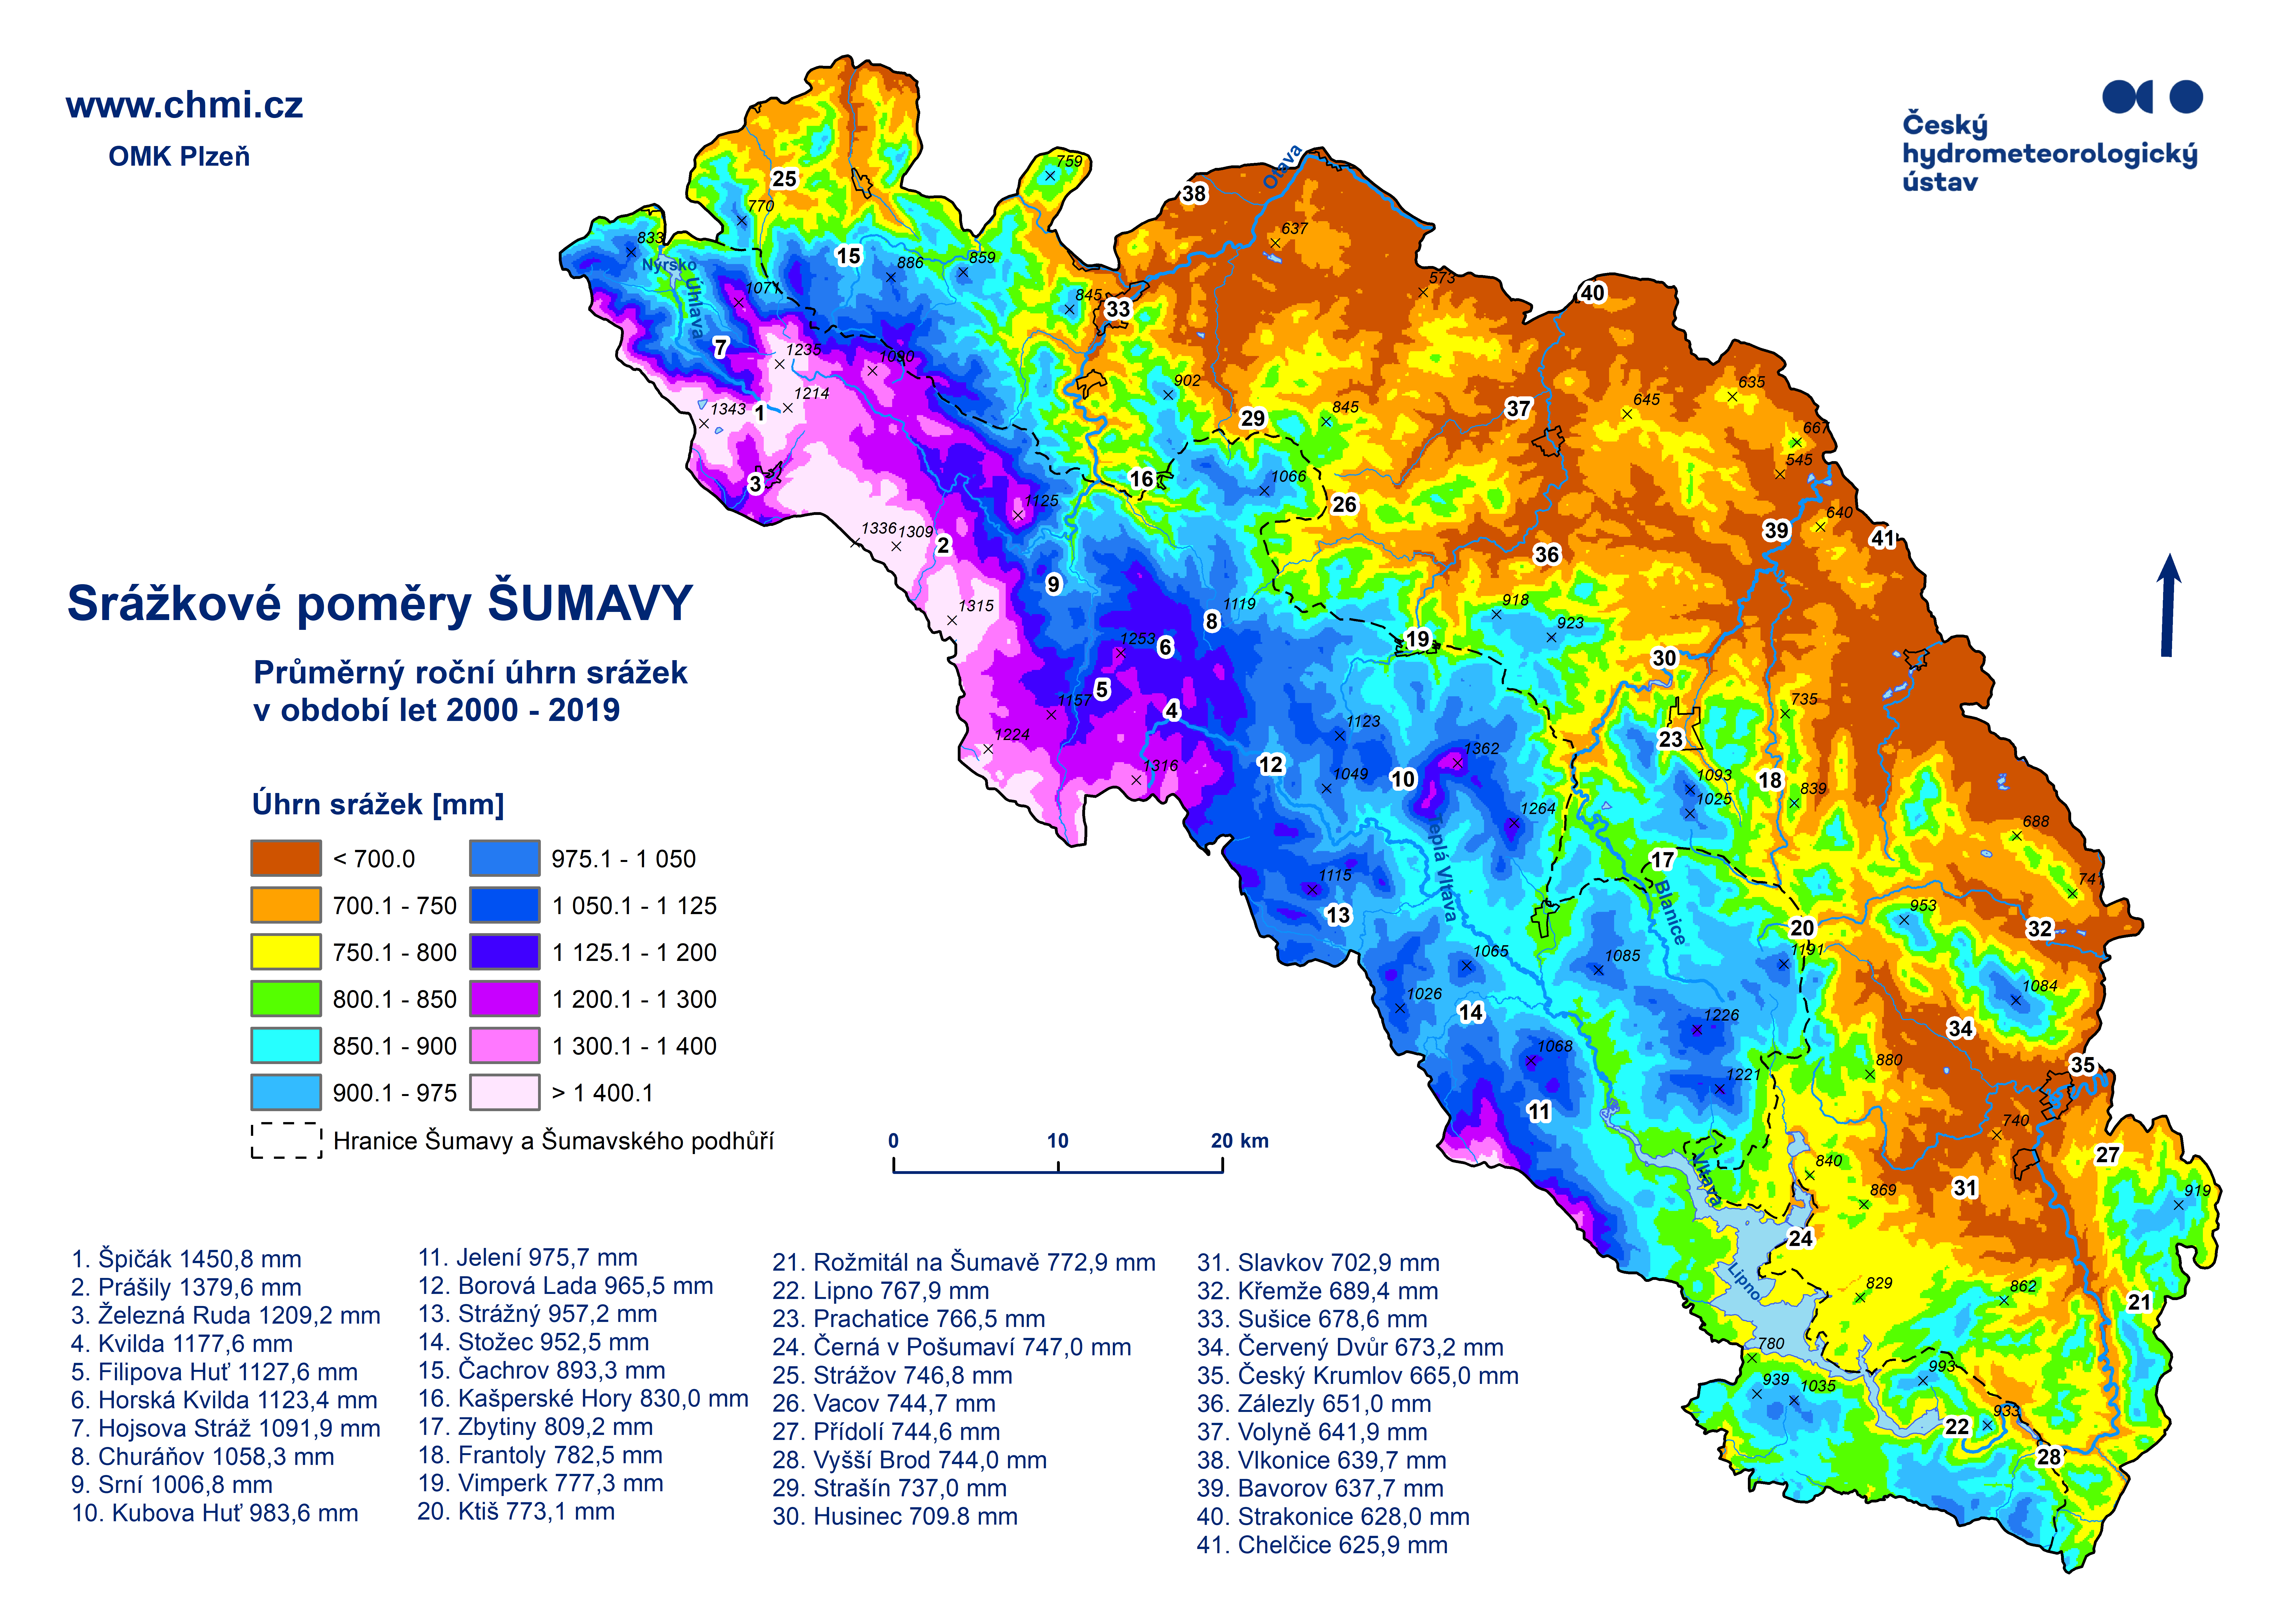
\includegraphics[width=0.95\textwidth]{img/ch1/srazkovepomerysumava.png}
	\caption{Srážkové poměry Šumavy \parencite{srazkovepomerysumava}, důležitá je pak hodnota $\SI{1058}{mm/rok}$ pro meteorologickou stanici Churáňov.}
	\label{fig:srazkovepomerysumava}
\end{figure}

\begin{figure}
	\centering
	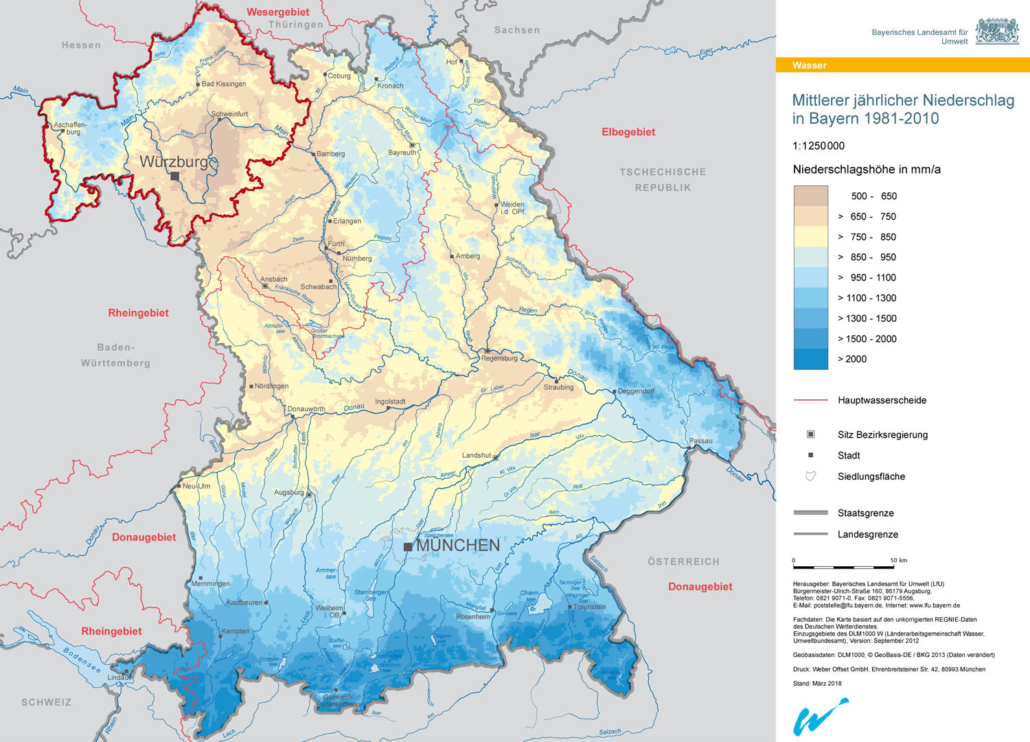
\includegraphics[width=0.95\textwidth]{img/ch1/srazkovepomerybavorskyles.png}
	\caption{Srážkové poměry v Bavorsku \parencite{srazkovepomerybavorskyles}}
	\label{fig:srazkovepomerybavorskyles}
\end{figure}

\clearpage

\section{Statistické metody}\label{chap:statistika}
%V kapitole \ref{chap:analysis} je vysvětleno jakým způsobem byla data zpracována. Zde nastíníme relevantní teorii.

\subsection{Lineární smíšený model}\label{chap:lme}
V maticovém zápisu je lineární smíšený model definován následovně: \parencite{mcleanrobert1991}
$$\boldsymbol{y} = \boldsymbol{X}\boldsymbol{\beta} + \boldsymbol{Z}\boldsymbol{u} + \boldsymbol{\epsilon},$$ \label{eq:linearmixedeffectmodel}
kde $\mathbf{y}$ je vektor pozorovaných hodnot, $\mathbf{\beta}$ je neznámý vektor hledaných fixní efektů, $\mathbf{u}$ je neznámý vektor náhodných efektů $\mathbf{\epsilon}$ je neznámý vektor náhodných chyb a matice $\mathbf{X}$ a $\mathbf{Z}$ jsou známé matice udávající vztah mezi pozorovanými hodnotami a fixními, resp. náhodnými efekty, jejichž velikost je daná počtem prediktorů a pozorování \parencite{mcleanrobert1991}.

U lineárního smíšeného modelu předpokládáme normální rozdělení residuí a očekáváme homoskedasticitu, tedy to, že rezidua nezávisí na hodnotě měřené veličiny \parencite{homoscedasticity}. Dále také předpokládáme data bez autokorelační a prostorové struktury a že máme normálně rozdělené náhodné efekty modelu \parencite{hefleytrevorj2017}. 

Pro lineární smíšený model můžeme definovat marginální a podmíněné $R^2$. Tato hodnota nám ukazuje kolik variance model vysvětluje. Marginální $R_m^2$ udává varianci vysvětlenou pomocí fixních efektů a podmíněné $R_c^2$ celého modelu.
\begin{gather}
	R_m^2 = \frac{\sigma_f^2}{\sigma_f^2+\sigma_{\alpha}^2+\sigma_{\varepsilon}^2},\\
	R_c^2 = \frac{\sigma_f^2+\sigma_{\alpha}^2}{\sigma_f^2+\sigma_{\alpha}^2+\sigma_{\varepsilon}^2},
\end{gather}
kde $\sigma_f^2$ je variance fixních efektů, $\sigma_{\alpha}$ je variance náhodných efektů a $\sigma_{\varepsilon}^2$ je variance pozorovaných hodnot \parencite{lmersquared}.

\subsection{ARMA model}
Pro modelování autokorelační struktury můžeme využít ARMA (autoregressive moving average) model. Ten je definován jako \parencite{wilsongranville2016}
\begin{gather*}
y_T = \epsilon_T + \sum_{i=1}^{p}u_i y_{T-i} + \sum_{i=1}^{q}\beta_i\varepsilon_{T-i},
\end{gather*}
kde $y_T$ časová řada, $\epsilon$ je náhodná chyba, $u_i$ jsou parametry náhodné proměnné a $\beta_i$ jsou parametry fixní proměnné. 

\subsection{F-test}
F-test může sloužit k testování statistické významnosti koeficientů lineárního (smíšeného) modelu. Mějme nulovou hypotézu, že všechny koeficienty modelu $\beta_i = 0\, \forall i$. Dále mějme alternativní hypotézu $\exists j, \beta_j\neq 0$. Spočteme $F$ statistiku jako podíl vysvětlené a nevysvětlené variance. Následně spočteme pomoctí statistického softwaru konfidenční interval $I$ a zavrhneme nulovou hypotézu pokud $F\notin I$ a určíme p-hodnotu. V programovacím jazyce \texttt{R}, můžeme použít například funkci \texttt{anova} \parencite{ftest}.

\subsection{Kvantil-kvantilový graf}
Pro srovnání dvou statistických rozdělení používáme kvantil-kvantilový graf. Na ose $x$ jsou kvantily jednoho rozdělení a na ose $y$ druhého. Pokud chceme zjistit, jestli nějaké datový soubor je blízký normálnímu rozdělení, vykreslíme proti sobě kvantily normálního rozdělení a kvantily datového souboru, čím blíže jsou hodnoty přímce $y(x)=x$, tím lépe odpovídá rozdělení normálnímu (až na násobek a konstantu rozdělení). Z kvantil-kvantilového grafu můžeme také například odhalit, jestli jsou hodnoty zešikmené nebo jestli lépe odpovídají bimodálnímu rozdělení \parencite{interpretqqplot}.

Testování normality nějakého rozdělení můžeme také použít formální testy jako například Shapiro-Wilkův test. Tuto možnost budeme diskutovat v metodách zpracování dat \ref{chap:analysis}. %\parencite{shapirowilk}. 

\subsection{Semivariogram}\label{chap:variogram}
Pro posouzení prostorové korelace dat využijeme metodu variogramu. Experimentální variogram nám určuje prostorovou závislost naměřených hodnot. V našem případě jde o hodnoty naměřených teplot neboli jejich rozdíl. Experimentální semivariogram může být definován například následovně

\begin{gather*}
	\gamma(\mathbf{h}) = \frac{1}{2m(\mathbf{h})}\sum_{i=1}^{m(\mathbf{h})}\left(t(\mathbf{x}_i) - t(\mathbf{x}_i+\mathbf{h})\right)^2,
\end{gather*}

kde v našem případě $t(\mathbf{x}_i)$ a $t(\mathbf{x}_i+\mathbf{h})$ jsou pozorované hodnoty (rozdílů) teplot na jednotlivých čidlech a $m(\mathbf{h})$ je počet párů teplot vzdálených od sebe o $\mathbf{h}$. Hodnota vzdálenosti $\mathbf{h}$ se tedy pohybuje od vzdálenosti dvou nejbližších čidel až po vzdálenost dvou nejvzdálenějších čidel. Variogram je typicky dvojnásobek semivariogramu tedy $2\gamma(\mathbf{h})$ \parencite{variogram}.

Podle článku \parencite{predictingforestmicroclimate} prostorová korelace průměrný denních teplot v heterogenním lese v severní Kalifornii přestává být významná ve vzdálenosti $\SI{4}{km}$ až $\SI{6}{km}$.

\subsection{Použitý software}
Pro zpracování dat jsme využívali primárně programovací jazyk \texttt{R}\parencite{Rlanguage} a jeho verzi \texttt{4.1.3}. Použili jsme následující baličky a knihovny pro přípravu a analýzu dat: \texttt{stringr}\parencite{stringr}, \texttt{e1071}\parencite{e1071}, \texttt{xlsx}\parencite{xlsx}, \texttt{geosphere}\parencite{geosphere}, \texttt{ggplot2}\parencite{ggplot2}, \texttt{lmtest}\parencite{lmtest}, \texttt{data.table}\parencite{data.table}, \texttt{lubridate}\parencite{lubridate}, \texttt{nlme}\parencite{nlme}, \texttt{forecast}\parencite{forecast}, \texttt{moments}\parencite{moments}, \texttt{profvis}\parencite{profvis} a \texttt{climate}\parencite{climate}. Pro otevření dat formátu \texttt{grib} a jejich transformaci z reanalýzy ERA5 jsme použili programovací jazyk \texttt{Python}, verzi \texttt{3.8.13}\parencite{Python} a knihovny \texttt{xarray}\parencite{xarray}, \texttt{numpy}\parencite{numpy}, \texttt{pandas}\parencite{pandas}, \texttt{cfgrib}\parencite{cfgrib} a \texttt{eccodes}\parencite{eccodes}. Pro vykreslení obrázku \ref{fig:rozlozenicidel} byl použit software \texttt{QGIS}, verze \texttt{3.10}\parencite{qgis}
